\documentclass[11pt]{article}

\usepackage{filecontents}
\begin{filecontents}{\jobname.bib}
@article{sneath1957application,
  title={The application of computers to taxonomy},
  author={Sneath, Peter HA},
  journal={Journal of general microbiology},
  volume={17},
  number={1},
  pages={201--226},
  year={1957},
  publisher={Soc General Microbiol}
}
\end{filecontents}

\usepackage{natbib}
\usepackage{adjustbox}
\usepackage{amsmath}
\usepackage[font=footnotesize]{caption}
\usepackage[dvipsnames]{xcolor}
\usepackage{geometry}
  \geometry{margin=1in}
\usepackage{framed}
\usepackage[breaklinks]{hyperref}
\usepackage{minibox}
\usepackage[compact]{titlesec}

\graphicspath{ {./figures/} }




\begin{document}


\noindent
\large
\begin{minipage}{0.5\textwidth}
\begin{flushleft} 
IB200, Spring 2016
\end{flushleft}
\end{minipage}
\begin{minipage}{0.5\textwidth}
\begin{flushright} 
\textit{University of California, Berkeley}
\end{flushright}
\end{minipage}

\vspace{0.5cm}


\begin{center}
\Large \textbf{Lab 04:} \\
Distance and parsimony inference using PAUP*; \\
UPGMA, neighbor-joining, bootstrap, and jackknife \\
\normalsize
\textit{Updated by Will Freyman}
\end{center}

\vspace{0.5cm}

\section{Before you begin}

Please download:

\begin{enumerate}
  \item PAUP*: download the \textbf{command-line binary} (not the GUI version) at: \\ 
        \url{http://people.sc.fsu.edu/~dswofford/paup_test/}
  \item Primate mitochondrial DNA: \\
        \url{http://ib.berkeley.edu/courses/ib200/labs/04/primate-mtDNA.nex}
\end{enumerate}

%\begin{verbatim}
%text editor
%Mesquite
%FigTree
%\end{verbatim}

\section{Introduction}

Today we will cover both distance and parsimony inference using the software PAUP*
and introduce two different methods of measuring uncertainty over
the phylogeny: the bootstrap and jackknife.
PAUP* (Phylogenetic Analysis Using Parsimony [*and other methods]) is 
supposedly pronounced “pop star”, and it 
can infer phylogenies using distance, parsimony, and likelihood. 
It is widely used (with over 40 \textit{thousand} citations),
however its author, David Swofford, has recently (2015) 
released the Bayesian phylogenetics software Phycas
with Paul Lewis and Mark Holder.




\section{Basic PAUP*}

Open PAUP*.
PAUP* takes a nexus (.nex) file as input. 
If you have your own sequence data you can use that, 
otherwise use the \texttt{primate-mtDNA.nex} file.
First set the working directory (like in R)
by typing \texttt{cd <directory>} where \texttt{<directory>}
is the full path to the directory in which you saved
the \texttt{primate-mtDNA.nex} file.
Now type \texttt{execute primate-mtDNA.nex}.

PAUP* will tell you a few things about the file (how many taxa and characters it has in it, what nucleotide ambiguity codons are being used). For instance, right now “R” is treated as either A or G for analytical purposes.
You can type \texttt{?} after a command to see a brief description of it. Check
out some other useful commands:

\begin{verbatim}
cstatus
showdist
showmatrix
tstatus
\end{verbatim}

\begin{framed}
\noindent
\textbf{Question 1:} \\
Use the commands above to explore the dataset.
What is the optimality criterion currently set to? Are these characters
ordered or unordered?
What is the distance between chimpanzees and humans? % 0.08929
\end{framed}

\section{Distance Methods}

Distance-based methods are mostly hierarchical clustering algorithms.
In fact, many major early contributions to clustering algorithms were
developed by phylogeneticists/pheneticists, for example single-linkage hierarchical clustering
was first introduced in \citet{sneath1957application}.

From lecture you have learned that distance-based methods are not the most theoretically justified of methods for inferring phylogenies, although clustering methods do have many other uses in statistics and computer science. 
They are by far the fastest way to find a tree. Whereas parsimony and likelihood methods have to search through tree space and compare the optimization of the character matrix on many trees, most distance methods use an algorithm to directly generate a tree from the distance matrix. This speed makes it very useful for genomics, where it is often necessary to generate tens of thousands of trees, but getting the exact tree each time is not as important as getting the right tree the vast majority of the time.


Change the optimality criteria to distance.
\begin{verbatim}
paup> set criterion = distance;
\end{verbatim}

\subsection{UPGMA}

UPGMA (Unweighted Pair Group Method with Arithmetic Mean) 
is a clustering algorithm for generating trees from a distance matrix. It assumes that the trees are ultrametric, meaning that the branch lengths obey the molecular clock. It approximates the least squares tree and is well behaved if the molecular clock is followed. Generate a UPGMA tree with branch lengths and save it:

\begin{verbatim}
paup> upgma brlens = yes treefile=upgmatree.tre;
\end{verbatim}

\subsection{Neighbor Joining}
Neighbor joining (NJ) is another clustering algorithm, but it does not assume the molecular clock. 
NJ has the mathematical property that if the distance matrix is correct, then the output tree will be correct.
NJ is currently the distance method with the best reputation and is thus the one most commonly used, although UPGMA is still used in a lot of genomics studies. The clustering algorithm of NJ is similar to that of UPGMA in that both replace pairs of OTUs with composite OTUs one after another. 
However, compared to UPGMA it is more complex. NJ uses the distance matrix to calculate
a $Q$ matrix that we won't go over here.
Generate a NJ tree with branch lengths and save it:

\begin{verbatim}
paup> nj brlens = yes treefile=njtree.tre;
\end{verbatim}


\begin{framed}
\noindent
\textbf{Question 2:} \\
What is the total branch length sum for your UPGMA tree? 
For your NJ tree? 
[HINT: Scroll back up through your PAUP window to find this information]
Examine these two trees in FigTree. 
What is the main difference between these two trees in terms of branch lengths?
\end{framed}

\section{Parsimony}

Parsimony is the optimality criterion that minimizes the number of changes on the tree. Unlike distance methods, it is a phylogenetic method that distinguishes between symplesiomorphy and synapomorphy. Change the optimality criteria to Parsimony.

\begin{verbatim}
paup> set criterion=parsimony
\end{verbatim}

Then, run a heuristic search:

\begin{verbatim}
paup> hs
\end{verbatim}

Then save your trees:

\begin{verbatim}
paup> savetrees file=parstree.tre
\end{verbatim}

Open this tree file in FigTree along with your UPGMA and NJ trees to examine them.

\begin{framed}
\noindent
\textbf{Question 3:} \\
Do the tarsiers fall out in the sample place in all your trees?
\end{framed}

\section{Estimate Support by Bootstrapping}

\begin{figure}
\centering
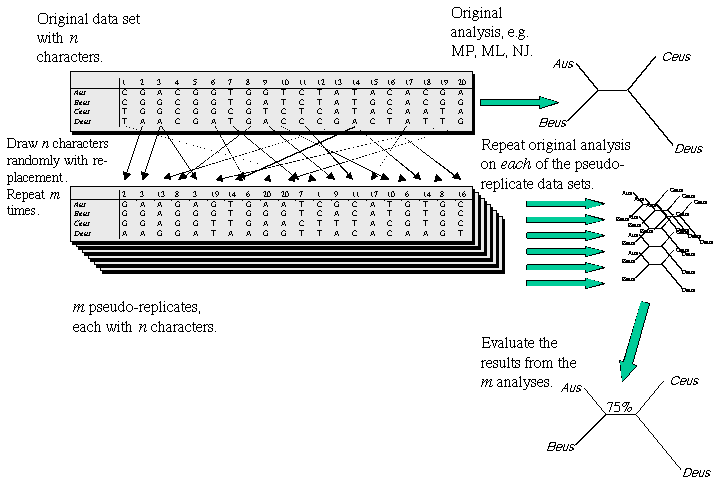
\includegraphics[width=0.7\textwidth]{bootstrap.png}
\caption{Bootstrap replicates. Image from \\ http://artedi.ebc.uu.se/course/X3-2004/Phylogeny/Phylogeny-Credibility/Phylogeny-Credibility.html}
\end{figure}

Okay, now let's figure out how well supported these groupings are. One measure of support is called the 
\textbf{bootstrap}. 
It works by choosing columns randomly from the matrix until it is has chosen the same number of columns as were in the original matrix. Because it returns to the original matrix each time it chooses a new column, some characters may be
represented several times in the bootstrap matrix, while others are omitted. This is known as resampling the data with replacement. In practice, although it is possible to randomize taxa, bootstrapping almost always randomizes characters. Bootstrapping calculates a support value for each node based on the fraction of samples that support that node. 
Bootstrap provides a number on each node ($0-100$). 
The highest support value is 100, while values below 70 are usually considered weak. Values below 50 aren't shown. In fact, branches below 50 are collapsed and shown as a polytomy. Bootstrap support is somewhat sensitive to the number of replicates used, but not terribly so.


Now let's run a bootstrap analysis with a hundred replicates, using a heuristic search for each replicate, 
and randomizing the order of taxa while building the trees on your data.
When it's done, PAUP will display a 50\% 
majority rule consensus tree from all 100 bootstrap runs. 
This type of consensus tree only shows clades that are present in more than 50\% of the primary trees.

\begin{verbatim}
paup> bootstrap nreps=100 search=heuristic /addseq=random;
\end{verbatim}

PAUP will also display a list showing the frequency of different taxon bipartitions (that is, how often out of the 100 replicates the taxa were grouped together.) 
If you look at the tree, you’ll see that Pan has a (3) after it and Gorilla has a (4). 
Look down the chart until you see a line where there is a * under 3 and 4, 
but not under any of the other numbers. 
The frequency on this line will be something like 47.70, 
which means these two taxa were grouped together in about 47.7 out of the 100 runs. 
Some of these numbers are fractional because some runs 
produced more than one most parsimonious tree.

Ok, now you may want to export the fancy new bootstrap values you just came up with. Well, luckily there is a way to do that:

\begin{verbatim}
paup> savetrees from=1 to=1 savebootp=nodelabels file=bootstrap.tre;
\end{verbatim}


Note that you must supply the tree numbers that you want to save (here, from 1 to 1, since there is only one bootstrap tree) and the file name you want to save to. You can view these node labels on the tree in FigTree or Mesquite.

\begin{framed}
\noindent
\textbf{Question 4} \\
Figure out a way to show your tree with bootstrap support in FigTree. 
Note: The program can be a bit glitchy for some reason so you may need to open the program first and 
then go to \texttt{File - Open} to select your file. 
Highlight the weakly supported \textit{Pan - Gorilla} clade and take a screenshot.
\end{framed}


\section{Estimate Support by Jackknifing}

Jackknifing is very similar to bootstrapping, but rather than resample the data, it uses subsets of the data. 
This is also described as resampling without replacement to create a smaller dataset. 
The purpose of this is to see if excluding certain characters has a big effect on the shape of the tree. 
(You can imagine that some 'outlier' character might have a disproportionate influence on the relationships that are reconstructed; 
jackknifing is an attempt to get around this.) 
Jackknifing is much less common in the literature than bootstrap support.

\begin{verbatim}
paup> jackknife nreps=100 search=heuristic /addseq=random;
\end{verbatim}

Export the jackknife values the same way you exported the bootstrap ones:

\begin{verbatim}
paup> savetrees from=1 to=1 savebootp=nodelabels file=jackknife.tre;
\end{verbatim}


\begin{framed}
\noindent
\textbf{Question 5} \\
Open your jackknife tree file in FigTree and show the jackknife values on the tree.
Then highlight the weakly supported clade \textit{Pan} and take a screen shot.
\end{framed}

\begin{framed}
\noindent
\textbf{Please email me the following:}
\begin{enumerate}
  \item The answers to questions 1-5.
  \item Screengrabs of your bootstrap and jackknife trees with support values and the \textit{Pan} clades highlighted.
\end{enumerate}
\end{framed}

\bibliographystyle{plainnat}
\bibliography{\jobname} 

\end{document}

